\documentclass[a4paper,12pt]{article}
\usepackage[utf8]{inputenc}
\usepackage[spanish]{babel}
\usepackage{graphicx}
\usepackage{libertine}
\renewcommand\familydefault{\sfdefault}
\usepackage[T1]{fontenc}
\usepackage[colorlinks=true,linkcolor=blue]{hyperref}
\usepackage[framed,numbered,autolinebreaks,useliterate]{mcode}

\parindent = 0mm

\author{Moisés Gautier Gómez}
\title{
\includegraphics[width=10cm]{logo_ugr.png} \\ 
\includegraphics[width=3cm]{fetch.png}\\ Práctica 3 - Teoría de la Señal y Comunicaciones 
}
\date{ }

\begin{document}
\maketitle
Ejercicios
%\lstinputlisting{genexp.m}

\begin{enumerate}
\item Utilizado Simulink se realizará un cuantificador uniforme de 4 bits para una señal sinusoidal de amplitud 1 y frecuencia 1 Hz. Se estudiará la forma de onda de la señal error así como la SNRQ y su relación con el número de bits de cuantificación para 3 y 2 bits. \\

La función de entrada será la función seno:
$$f(t) = \sin(2\pi t)$$
con una amplitud 1 y una frecuencia de 1 Hz.

$\Delta$ es el tamaño del cuanto y depende del rango dinámico de la señal (máxima amplitud) y del número de bits utilizados para la codificación, por tanto:
$$ \Delta = \frac{2 \cdot X_{max}}{2^B}\ siendo\ X_{max} = 1 $$
La SNRQ se define como la relación señal-ruido de cuantificación y es una medida indicativa de la bondad de la cuantificación. Se define como la razón entre la varianza de la señal de entrada y la varianza de la señal error de cuantificación:
$$SNRQ = 10 log_{10}(\frac{\sigma^{2}_{x}}{\sigma^{2}_{e}})$$
En el archivo SNRQ.m se ha implementado la función correspondiente:\\
\lstinputlisting{SNRQ.m}
Cuantificador\\
\begin{center}
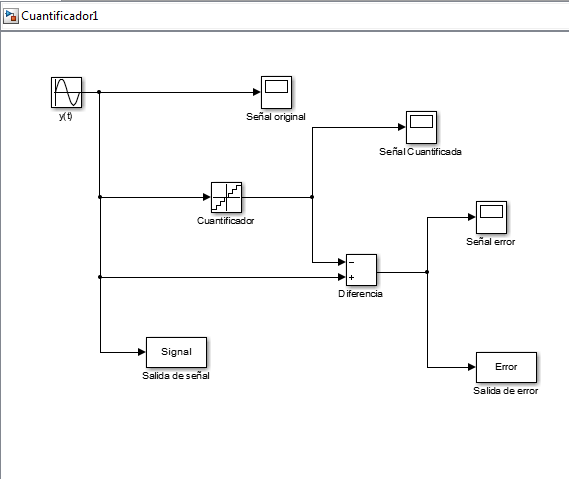
\includegraphics[width=.9 \textwidth]{Cuantificador-1.png}
\end{center}
Simulaciones:\\
\begin{center}
Señal original\\
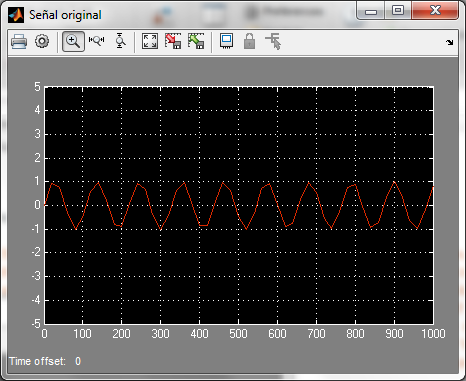
\includegraphics[width=.65 \textwidth]{signal-original.png}
\end{center}
Con 4 bits\\
$$\Delta = \frac{2 \cdot X_{max}}{2^B} = \frac{2 * 1}{2^4} = 2^{-3} = 0,125;\ SNRQ = 26,4493 $$
\begin{center}
Señal 4 bits (cuantificada)\\
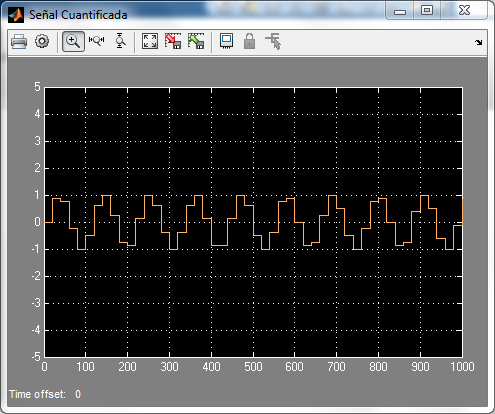
\includegraphics[width=.65 \textwidth]{signal-cuantificada-4-bits.png}\\
Señal 4 bits (error)\\
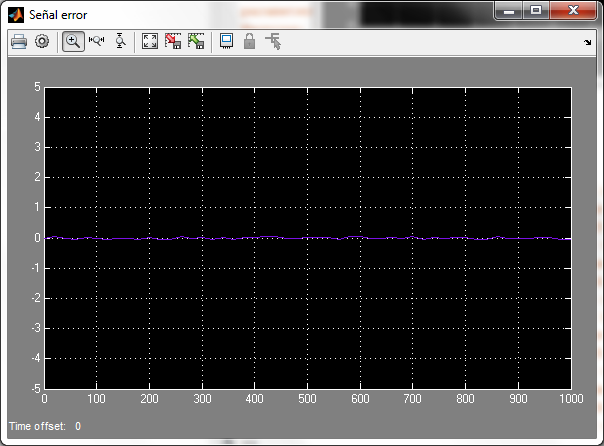
\includegraphics[width=.65 \textwidth]{signal-error-4-bits.png}
\end{center}
Con 3 bits
$$\Delta = \frac{2 \cdot X_{max}}{2^B} = \frac{2 * 1}{2^3} = 2^{-2} = 0,25;\ SNRQ = 20,6633 $$\\
\begin{center}
Señal 3 bits (cuantificada)\\
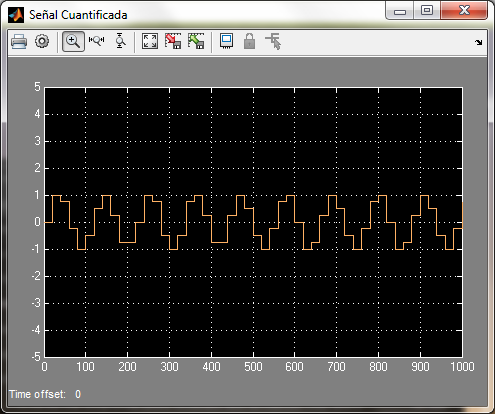
\includegraphics[width=.65 \textwidth]{signal-cuantificada-3-bits.png}\\
Señal 3 bits (error)\\
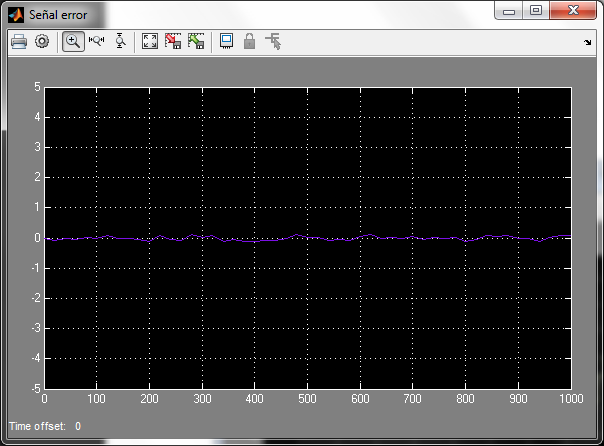
\includegraphics[width=.65 \textwidth]{signal-error-3-bits.png}\\
\end{center}
Con 2 bits
$$\Delta = \frac{2 \cdot X_{max}}{2^B} = \frac{2 * 1}{2^2} = 2^{-1} = 0,5;\ SNRQ = 14,8274 $$\\
\begin{center}
Señal 2 bits (cuantificada)\\
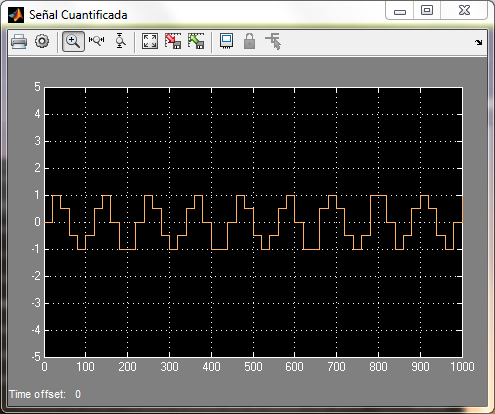
\includegraphics[width=.65 \textwidth]{signal-cuantificada-2-bits.png}\\
Señal 2 bits (error)\\
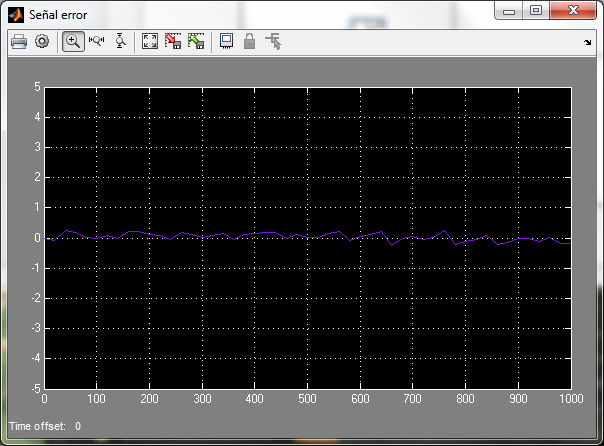
\includegraphics[width=.65 \textwidth]{signal-error-2-bits.png}
\end{center}

\item Utilizando el esquema de cuantificación diseñado anteriormente se estudiará el efecto de la cuantificación uniforme de una señal de voz (que se tomará del fichero asci signal.asc). Esta señal esta cuantificada con 16 bits, se propone la recuantificación a 12, 10 y 8 bits de la siguiente manera:
\begin{enumerate}
\item 12 bits: el cuanto se fija a $2^{16-12} = 16$.
\item 10 bits: el cuanto se fija a $2^{16-10} = 64$.
\item 8 bits: el cuanto se fija a $2^,{16-8} = 256$.
\end{enumerate}
Estudie la SNRQ de cuantificación para cada uno de los casos y reproduzca la señal cuantificada en la tarjeta de audio. Comente los resultados.

Para realizar este ejercicio he realizado una función que guarda los valores de la señal proveniente del archivo a un tipo matriz[tiempo,valor] en el espacio de trabajo de Matlab.

\lstinputlisting{cargar.m}

Cuantificador:\\
\begin{center}
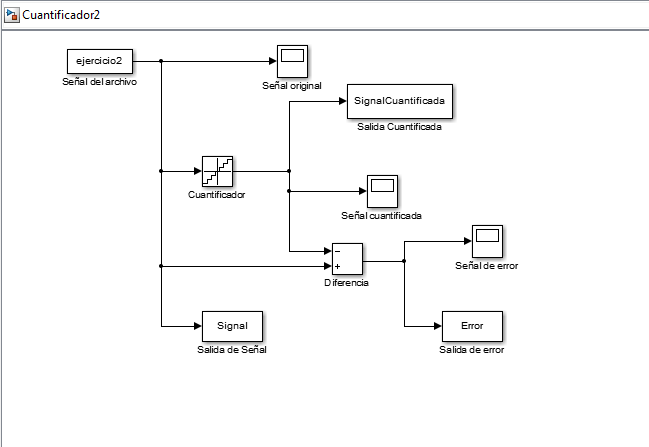
\includegraphics[width=.9 \textwidth]{Cuantificador-2.png}\\
\end{center}

Simulaciones:\\
Con 12 bits.
$$\Delta = 16;\ SNRQ = 55,6538$$
Con 10 bits.
$$\Delta = 64;\ SNRQ = 44,3696$$
Con 8 bits.
$$\Delta = 256;\ SNRQ = 33,2319$$

En la señal original se escucha la secuencia 39920361, y al cuantificar podemos comprobar que se escucha la misma secuencia de igual forma.

\item Usando simulink, diseño un cuantificador ley $\mu$ para la señal de voz (signal.asc).

Para calcular la señal de entrada, emplearemos la siguiente función:
$$F[x(n)] n = X_{max} \cdot \frac{log \bigl[ 1 + \mu \frac{|x(n)|}{X_{max}}\bigl]}{log(1 + \mu)} \cdot sig[x(n)]$$
Con $X_{max} = 2^{15} = 32768$ y $\mu = 255$. Así pues tenemos que:
\begin{eqnarray*}
F[x(n)] n & = & 32768 \cdot \frac{log \bigl[ 1 + 255 \frac{|x(n)|}{32768}\bigl]}{log(1 + 255)} \cdot sig[x(n)] \\ & = & 5909,3 \cdot log(1 + 0,0078 \cdot |x(n)|) sig[x(n)] 
\end{eqnarray*}

La señal cuantificada se calcula aplicando la inversa de esta función:
$$ y(n) = 5909,3 \cdot log(1 + 0,0078 \cdot |x(n)|) \cdot sig[x(n)] $$
$$ \frac{|y(n)|}{5909,3} = log(1 + 0,0078 \cdot |x(n)|) $$
$$ e^{\bigl( \frac{|y(n)|}{5909,3} \bigl)} = 1 + 0,0078 \cdot |x(n)| $$
$$ \frac{e^{\bigl( \frac{|y(n)}{5909,3} \bigl)} - 1}{0.0078} = |x(n)| $$
$$ F^{-1} [y(n)] = \frac{e^{\bigl( \frac{|y(n)|}{5909,3} \bigl)} - 1}{0,0078} \cdot sig[y(n)] $$

Cuantificador: \\

\begin{center}
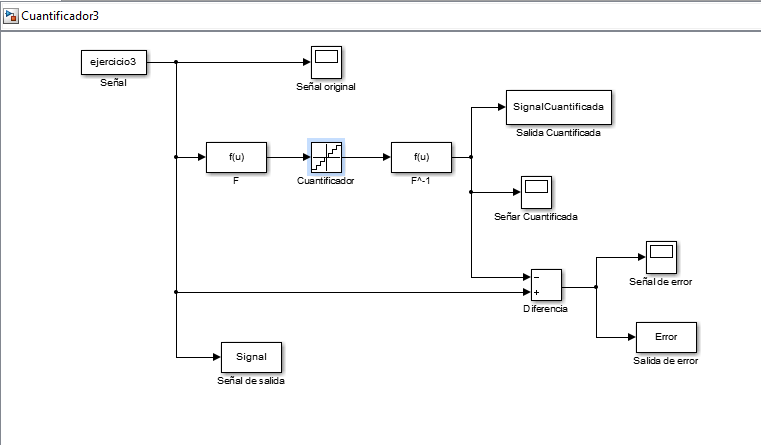
\includegraphics[width=.9 \textwidth]{Cuantificador-3.png}\\
\end{center}

\item Calcule la SNR para 12, 10 y 8 bits de cuantificación.

Como en el siguiente ejercicio tendremos que comparar los datos obtenidos aquí con los obtenidos en el ejercicio 2, utilizaré los mismos cuantos.

Simulaciones:

Con 12 bits.
$$ \Delta = 16;\ SNRQ = 61,2672 $$
Con 10 bits.
$$ \Delta = 64;\ SNRQ = 55,1883 $$
Con 8 bits.
$$ \Delta = 256;\ SNRQ = 37,4841 $$

\item Compare los resultados con los obtenidos en el apartado anterior.

Lo que nos puede llamar la atención en primera instancia es que para los valores de SNRQ se obtiene un valor mayor en cuantificación logarítmica que en cuantificación uniforme, de ahí que la aproximación sea mejor. \\

Así pues, observando las gráficas de error, en cuantificación uniforme el error es muy parecido para todas las amplitudes, mientras que en cuantificación logarítmica, el error es mayor cuanto mayor es la amplitud.
\end{enumerate}
\end{document}

